\newpage
\section{Funktionsmuster}
In diesem Abschnitt werden für gewisse Teilfunktionen des Roboters Funktionsmuster oder Prototypen erstellt. Damit können die Bewegungsabläufe und die technische Machbarkeit veranschaulicht werden. Ebenfalls können Probleme frühzeitig identifiziert und behoben werden.
\subsection{Piktogrammerkennung mit CNN}
\label{sec:piktogrammerkennung-mit-cnn}
% vereinfachen ("dobbelisecher")
Das Ziel dieses Funktionsmusters ist es in erster Linie, Erfahrung zu sammeln mit OpenCV, Keras, TensorFlow und der Piktogrammerkennung mit einem Convolutional Neural Network (CNN). Als CNN wurde eine vereinfachte Version der VGGNet Architektur gewählt.
Der Programmcode der Pythonscripts ist auf Github\footnote{https://github.com/randombenj/hslu-pren1/tree/master/pictogram\_detection} wie auch in Anhang zu finden.

\subsubsection{Trainingsdaten}
Die Abbildung \ref{fig:deep-learning-dataset} zeigt einen Ausschnitt aus dem deep learning Datenset.

\begin{figure}[H]
  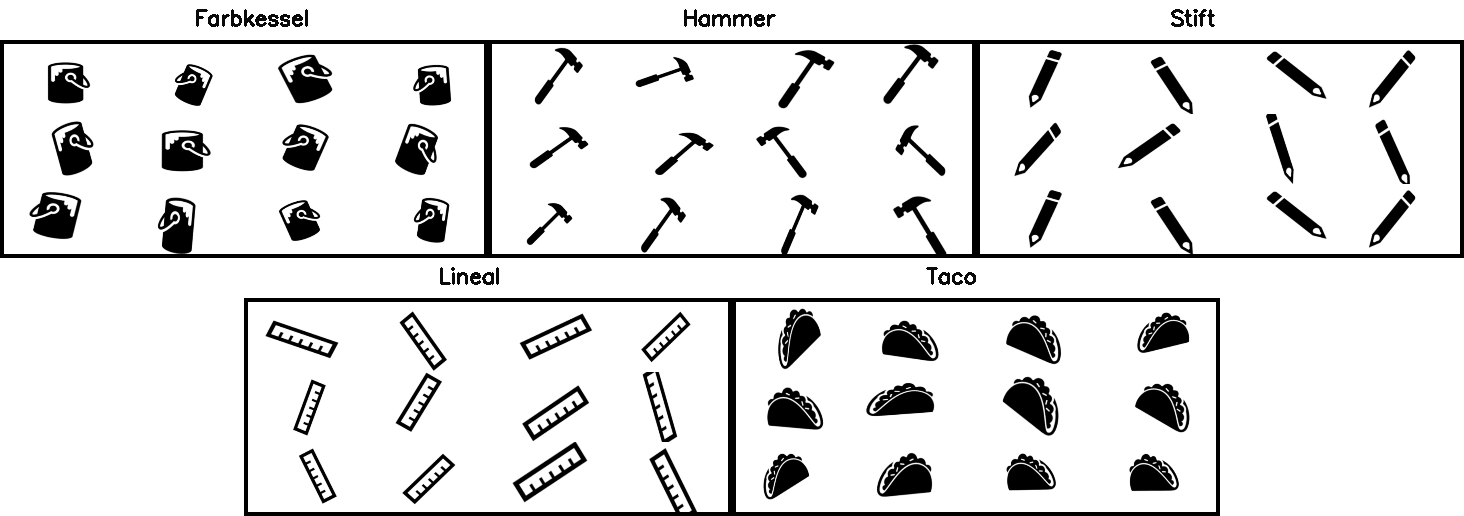
\includegraphics[width=1.0\textwidth]{img/piktogrammerkennung/collage.png}
  \centering
  \caption{Eine Bildmontage des multi-class deep learning dataset.}
  \label{fig:deep-learning-dataset}
\end{figure} 
   
Das Datenset besteht aus 500 Bildern über fünf Kategorien.
\begin{itemize}
    \item Hammer Piktogramm (100 Bilder)
    \item Farbkessel Piktogramm (100 Bilder)
    \item Lineal Piktogramm (100 Bilder)
    \item Bliestift Piktogramm (100 Bilder)
    \item Taco Piktogramm (100 Bilder)
 \end{itemize}
 
Die Trainingsdaten sind auf die Bilder in der Aufgabenstellung beschränkt. Um das Datenset zu vergrössern werden aus den original Piktogrammen mithilfe von Dataaugmentation viele leicht abgeänderte Versionen erstellt. Das Ziel dieses CNN ist, dass es anhand dieser Trainingsdaten die Piktogramme in der realen Welt korrekt klassifizieren kann. %für nicht informatiker verständlich machen

\subsubsection{Trainingsergebnisse}
Wie im Plot (Abbildung \ref{fig:trainingsergebnisse}) ersichtlich, wurde das CNN über 100 Epochs traniert und erreichte:
\begin{itemize}
    \item 99.9\% multi-label Klassifikationsgenauigkeit mit den Trainingsdaten (train\_acc)
    \item 98.9\% multi-label Klassifikationsgenauigkeit mit den Testdaten (val\_acc)
 \end{itemize}
 
\begin{figure}[H]
  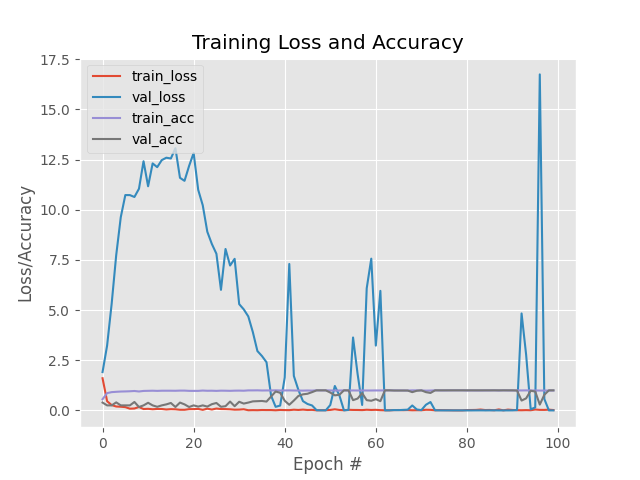
\includegraphics[width=0.7\textwidth]{img/piktogrammerkennung/trainingsergebnisse_piktogram.png}
  \centering
  \caption{Trainingsergebnisse des Funktionsmusters Piktogrammerkennung}
  \label{fig:trainingsergebnisse}
\end{figure} 
   
\subsubsection{Tests}
Um die Effektivität des Trainings zu testen werden verschiedenen Testbilder an das CNN übergeben. Das Diagramm kann die Originalbilder mit weissem Hintergrund voneinander unterscheiden, wie in der Abbildung \ref{fig:erfolgreiche-klassifikation-mit-cnn-1} und \ref{fig:erfolgreiche-klassifikation-mit-cnn-2} ersichtlich ist. Sobald sich jedoch eine Umgebung im Hintergrund des Bildes befindet, werden die Klassifizierungen sehr unpräzise. Die Abbildung \ref{fig:fehlerhafte-klassifikation-mit-cnn-1} zeigt eine fehlerhafte Klassifizierung.

\begin{figure}[H]
  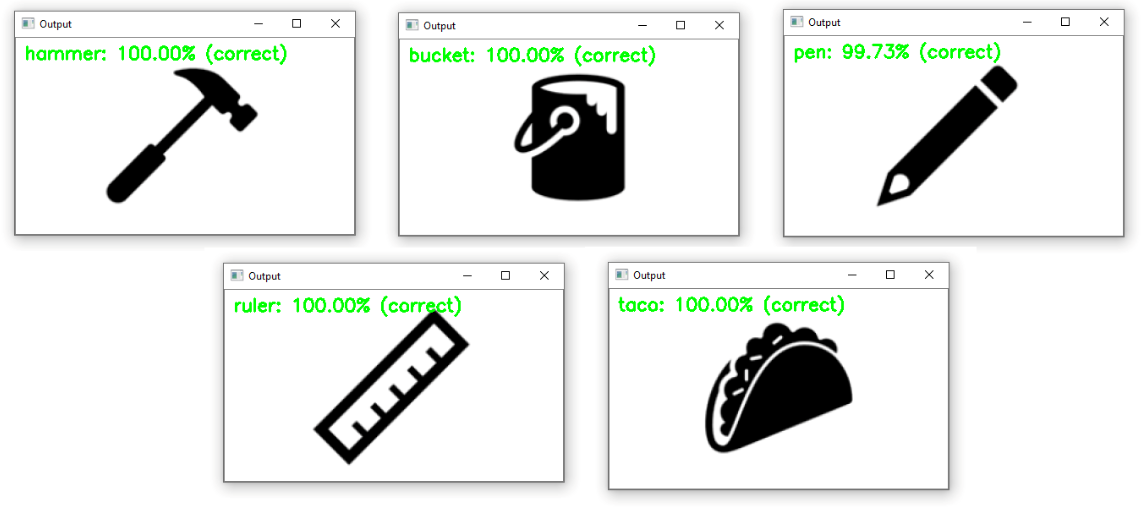
\includegraphics[width=1.0\textwidth]{img/piktogrammerkennung/collageCNN.PNG}
  \centering
  \caption{Erfolgreiche Ergebnisse der Piktogrammklassifikation}
  \label{fig:erfolgreiche-klassifikation-mit-cnn-1}
\end{figure}
   
\begin{figure}[H]
  \centering
  \begin{minipage}[t]{0.45\linewidth}
  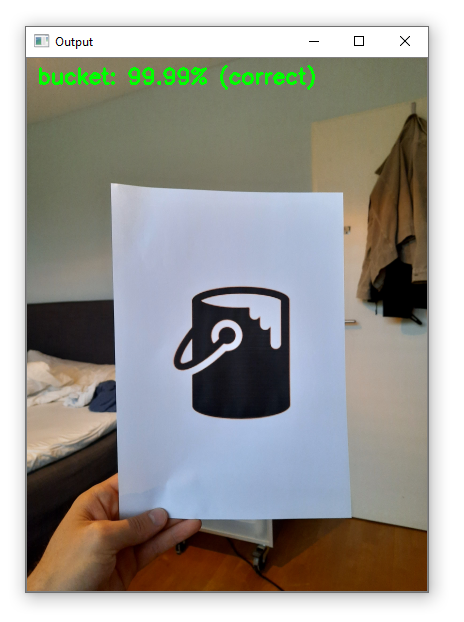
\includegraphics[width=0.7\textwidth]{img/piktogrammerkennung/classifiedBucketBG.PNG}
  \caption{Erfolgreiche Farbkesselklassifizierung mit Hintergrundumgebung}
  \label{fig:erfolgreiche-klassifikation-mit-cnn-2}
  \end{minipage} 
  \hfill
  \begin{minipage}[t]{0.45\linewidth}
  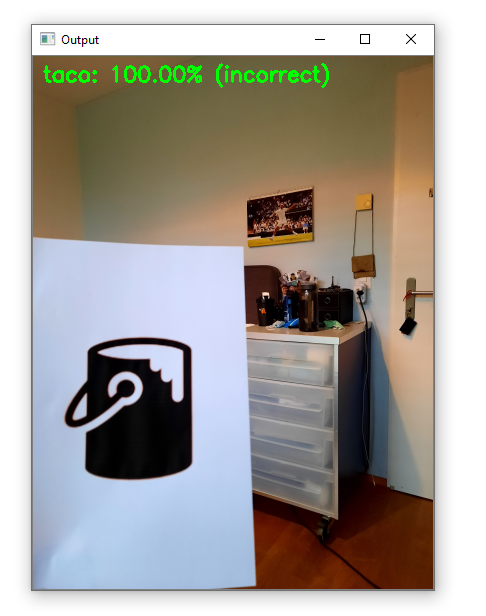
\includegraphics[width=0.7\textwidth]{img/piktogrammerkennung/notClassifiedBucketBG.PNG}
  \caption{Fehlgeschlagene Farbkesselklassifizierung mit viel Hintergrundumgebung}
  \label{fig:fehlerhafte-klassifikation-mit-cnn-1}
  \end{minipage}
\end{figure}

\subsubsection{Fazit}
Dieses Funktionsmuster hat gezeigt, dass die Piktogramme bereits mit wenigen und simplen Testdaten mit einer sehr hohen Wahrscheinlichkeit korrekt klassifiziert werden. Vorausgesetzt, die Piktogramme sind mit schwarz auf weissem Hintergrund abgebildet und es befindet sich sonst nichts im Hintergrund. Der Ansatz, die Piktogramme mithilfe eines CNN mit einer vereinfachten VGGNet-Architektur zu erkennen, könnte also weiter verfolgt werden.  

Da die Piktogramme in der Realität jedoch nicht einfach schwarz auf weiss und ohne Hintergrundumgebung vorzufinden sind, könnte man für eine korrekt Identifizierung folgende Ansätze weiterverfolgen:
\begin{itemize}
    \item Mehr Trainingsdaten
    \item Breiter diversivizierte Trainingsdaten (z.B. mit passendem Hintergrund)
    \item Input an den Traingsdaten anpassen durch Herausfiltern der Region of interest (ROI)
    \item Anderes deep learning Modell verwenden
 \end{itemize}
 
Jedoch hat sich im Daily-Standup mit dem Dozenten herausgestellt, dass machine learning nicht der richtige Lösungsansatz für die endliche Problemstellung der Piktogrammerkennung ist! 

Da man lediglich fünf, bereits im Vorfeld bekannte Piktogramme erkennen muss, kann man das mit sogenanntem Template Matching \cite{OpenCV-Template-Matching} realisieren. Hierbei werden Inputdaten mit den verschiedenen Templates, in unserem Fall die fünf Piktogramme, abgeglichen. Dabei wird versucht die verschiedenen Templates in den Inputdaten zu erkennen. 


\subsection{Hindernisserkennung}
\label{sec:hindernisserkennung-funktinosmuster}
Um die Treppe besteigen zu können ohne in die Hindernisse hineinzufahren, müssen
diese zuerst erkannt werden. Wie bereits bei anderen Komponenten wird auch hier versucht, eine möglichst simple Lösung zu finden.
Als erstes wird evaluiert, wie gut die Hindernisse mit einer Kamera und simpler Bildverarbeitung wie beispielsweise mittels OpenCV \cite{OpenCV}, erkannt werden
können.

Eine erste Idee ist die Ziegelsteine mittels Farbe zu erkennen. Diese Methode birgt natürlich das Risiko, dass bei unterschiedlicher Belichtung die Farben unterschiedlich wahrgenommen werden. Die Belichtung ist ein allgemeines Problem, tritt aber bei dieser Methode stärker hervor.

Die folgenden Beispiele zeigen die Resultate der auf Farbe basierenden 
Hinderniserkennung. Der sourcecode ist auf GitHub\footnote{https://github.com/randombenj/hslu-pren1/blob/master/research/obstacle-detection.ipynb} zu finden.

\begin{figure}[H]
  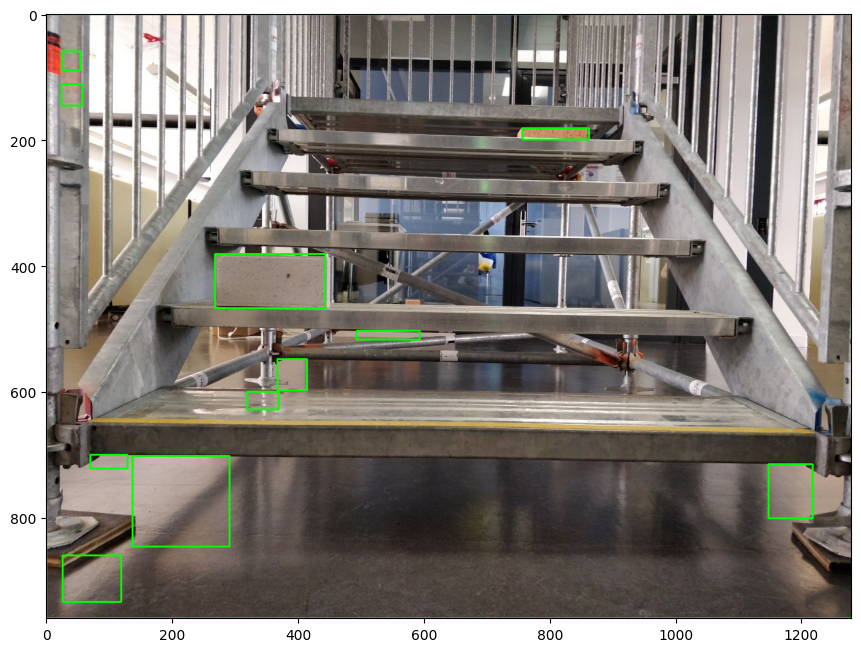
\includegraphics[width=1.0\textwidth]{img/hinderniserkennung/color-detection1.png}
  \centering
  \caption{Hinderniserkennung mit Farbdetektierung 1}
  \label{fig:color-detection-1}
\end{figure}

\begin{figure}[H]
  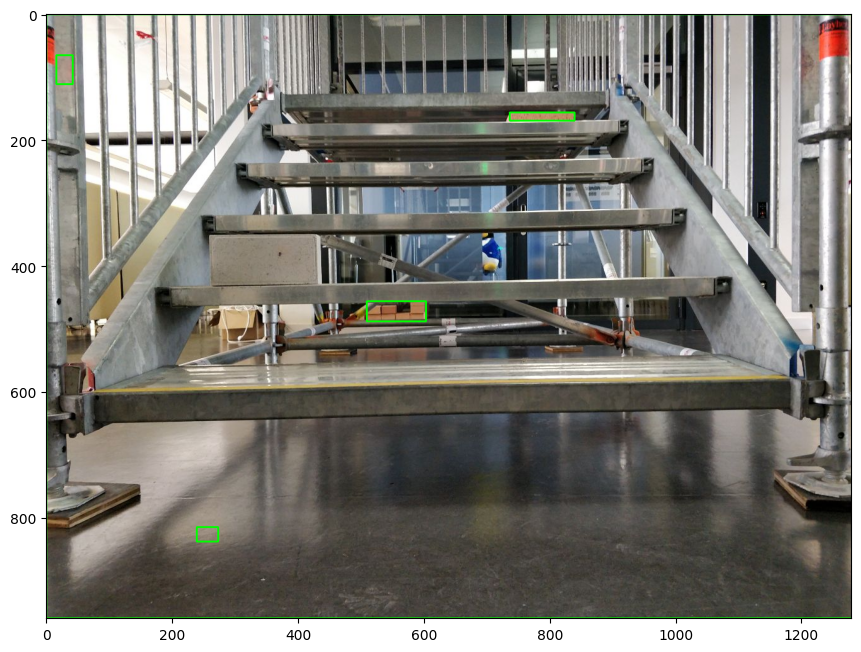
\includegraphics[width=1.0\textwidth]{img/hinderniserkennung/color-detection2.png}
  \centering
  \caption{Hinderniserkennung mit Farbdetektierung 2}
  \label{fig:color-detection-2}
\end{figure}

In Abbildung \ref{fig:color-detection-1} und \ref{fig:color-detection-2} ist ersichtlich, dass das Resultat bereits bei dem auf die Lichtverhältnisse optimierten
Code nicht besonders gut ist. Dies ist dementsprechend keine Option um
zuverlässig Hindernisse zu erkennen.

Um die Resultate zu verbessern, sollten unnötige Informationen weggelassen werden.
Unter der Annahme dass wir es bereits mit der fertigen Treppe zu tun haben
und uns zuverlässig immer an der gleichen Stelle vor der Treppe
aufstellen können, kann man bestimmte Ausschnitte aus dem Bild herausschneiden
welche für die Hinderniserkennung relevant sind.

Unter der Annahme, dass sich der Roboter an immer genau der gleichen stelle vor der Treppe positionieren kann,
und sich die Konfiguration der Treppe nicht ändert, können die Treppenstufen vom Bild wie in Abbildung \ref{fig:extracted-stairs} ausgeschnitten werden.
\begin{figure}[H]
  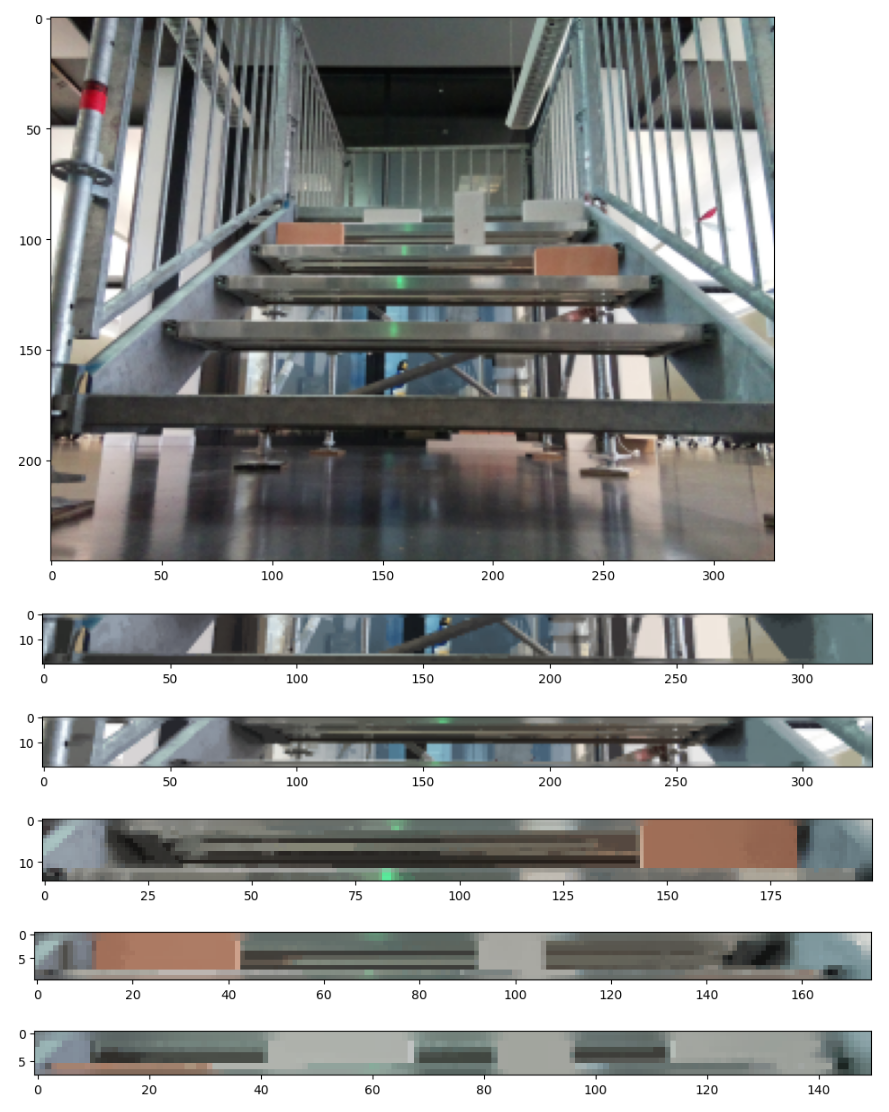
\includegraphics[width=1.0\textwidth]{img/hinderniserkennung/extracted-stairs.png}
  \centering
  \caption{Treppenstufen vom Bild ausgeschnitten}
  \label{fig:extracted-stairs}
\end{figure}

Ein grosses Problem bei dieser Methode ist, dass schon bei geringen Abweichungen der Position
des Roboters, die Resultate sehr ungenau werden. 
Zusätzlich ist wie auf Abbildung \ref{fig:extracted-stairs} zu erkennen ein Ziegelstein über zwei Treppenstufen ragend nicht richtig zugeordnet werden kann.

Für eine zuverlässige Hinderniserkennung auf der Treppe muss also auf eine Objekterkennungmethode mit beispielsweise einer 
Tiny-YOLO \cite{YOLOv3} Convolutional Neural Network (CNN) Architektur zurückgegriffen werden.

\subsection{Orientierung auf der Treppenstufe}
\label{sec:orientierung-auf-treppenstufe-funktionsmuster}
Sobald sich der Roboter auf einer Treppenstufe befindet und ein Ziegelstein das Erklimmen der nächsten Stufe verhindert, muss dieser seitlich auf der Treppenstufe traversieren können. Bei dieser seitlichen Bewegung besteht das Risiko\footnote{Siehe Risikomanagement im Anhang}, dass der Roboter vom Kurs ab kommt und eine Treppenstufe runter stürzt.
Deshalb ist geplant, die seitliche Bewegung mithilfe der Kamera zu kontrollieren. Somit ist es möglich, einem Abkommen vom Kurs rechtzeitig entgegen zu wirken.

Mithilfe dieses Funktionsmusters soll geprüft werden, ob es möglich ist, mit Hilfe der Kamera die eigene Position auf der Treppenstufe zu erkennen und so auf Kurs zu bleiben. 

\subsubsection{Testdaten}
Zum Testen werden verschiedene Bilder aus ungefähr 15 cm Höhe geschossen, welche das Blickfeld des Roboters beim Verschieben auf einer Treppenstufe simulieren sollen.

\subsubsection*{Aufbereitung der Bilder}
\label{sec:aufbereitung-der-bilder}
Um sich nun zu orientieren wird versucht Kanten und Linien in den Testdaten zu erkennen, welchen der Roboter folgen könnte. Um potentielle Kanten auszulesen, werden folgende Verarbeitungsschritte angewandt:
\begin{enumerate}
    \item Verkleinerung
    \item In Graustufen konvertieren
    \item Verzerren
    \item Erkennen von Kanten (Canny edge detection oder Threshold)
    \item Maskieren (Dieser Schritt sollte bereits zu beginn durchgeführt werden, um Ressourcen zu sparen)
    \item Finden von Linien (Hough Transform)
    \item Zeichnen der Linien
\end{enumerate}
Für das erkennen der Kanten werden zwei verschiedenen Techniken angewandt. Zum einen der Canny Edge Detection Algorithmus\cite{OpenCV-Canny}. Dieser Algorithmus erkennt Kanten auf einem Bild und färbt diese weiss ein. Je nach Justierung (mithilfe von zwei Parametern) werden mehr oder weniger Kanten erkannt. Die nachfolgende Abbildung \ref{fig:bildverarbeitungsschritte-canny-edge} visualisiert die einzelnen Bildverarbeitungsschritte basierend auf Canny Edge Detection.
\begin{figure}[H]
  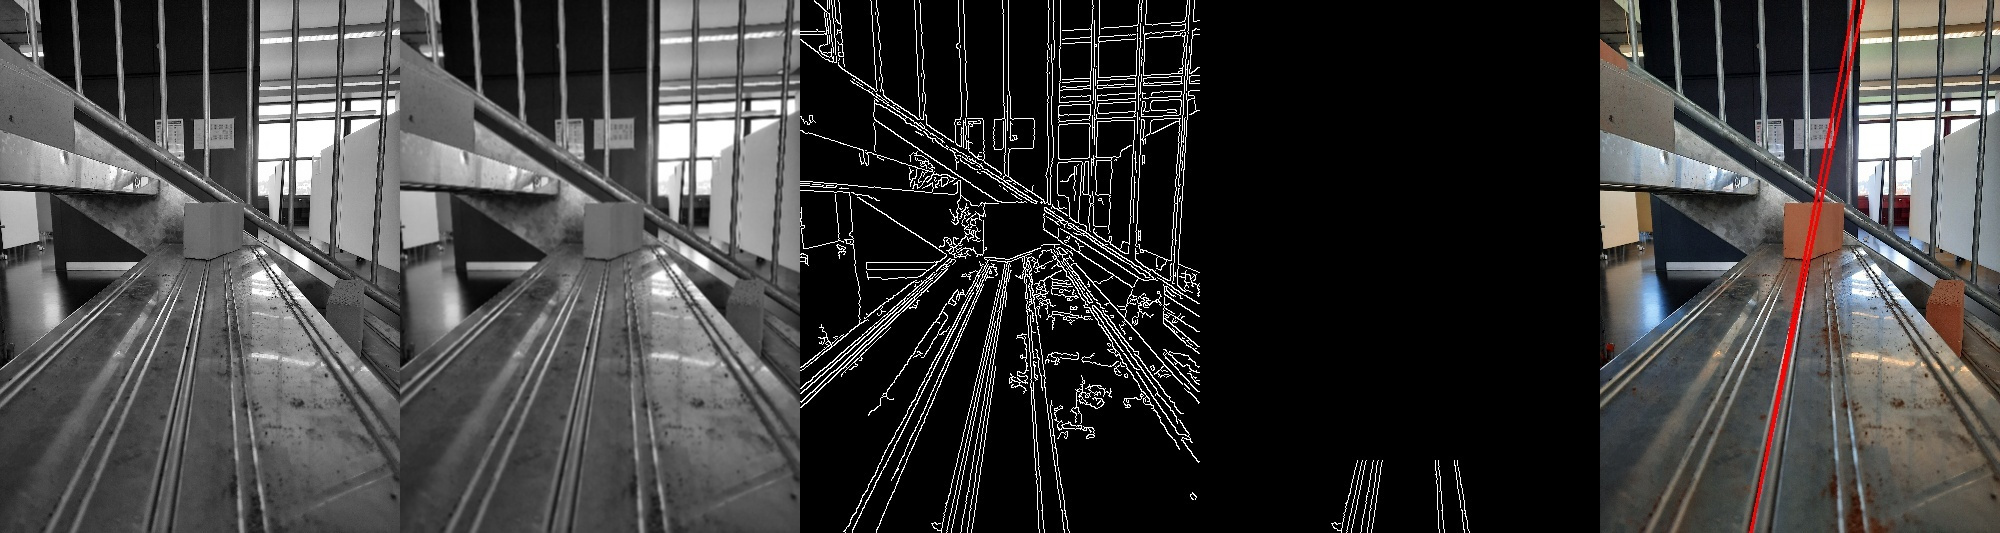
\includegraphics[width=1.0\textwidth]{img/orientierung-treppenstufe/collageCanny.jpg}
  \centering
  \caption{Bilverarbeitungschritte des Funktionsmusters für die Orientierung auf einer Treppenstufe mit Edge Detection}
  \label{fig:bildverarbeitungsschritte-canny-edge}
\end{figure}
  
Zum anderen wird Gebrauch vom Thresholding Algorithmus\cite{OpenCV-Threshold} gemacht. Dieser Algorithmus setzt voraus, dass das Bild in Graustufenform vorliegt, weil somit das Bild nur noch eine Farbdimension (0-255) enthält. Sobald dies der Fall ist, werden alle Pixelwerte oberhalb der Grenze z.B. auf Schwarz und alle die unterhalb der Grenze liegen auf z.B. Weiss gefärbt. Die Grenze kann beim Funktionsaufruf als Parameter übergeben werden. Die nachfolgende Abbildung \ref{fig:bildverarbeitungsschritte-threshold} visualisiert die einzelnen Bildverarbeitungsschritte basierend auf Thresholding.
\begin{figure}[H]
  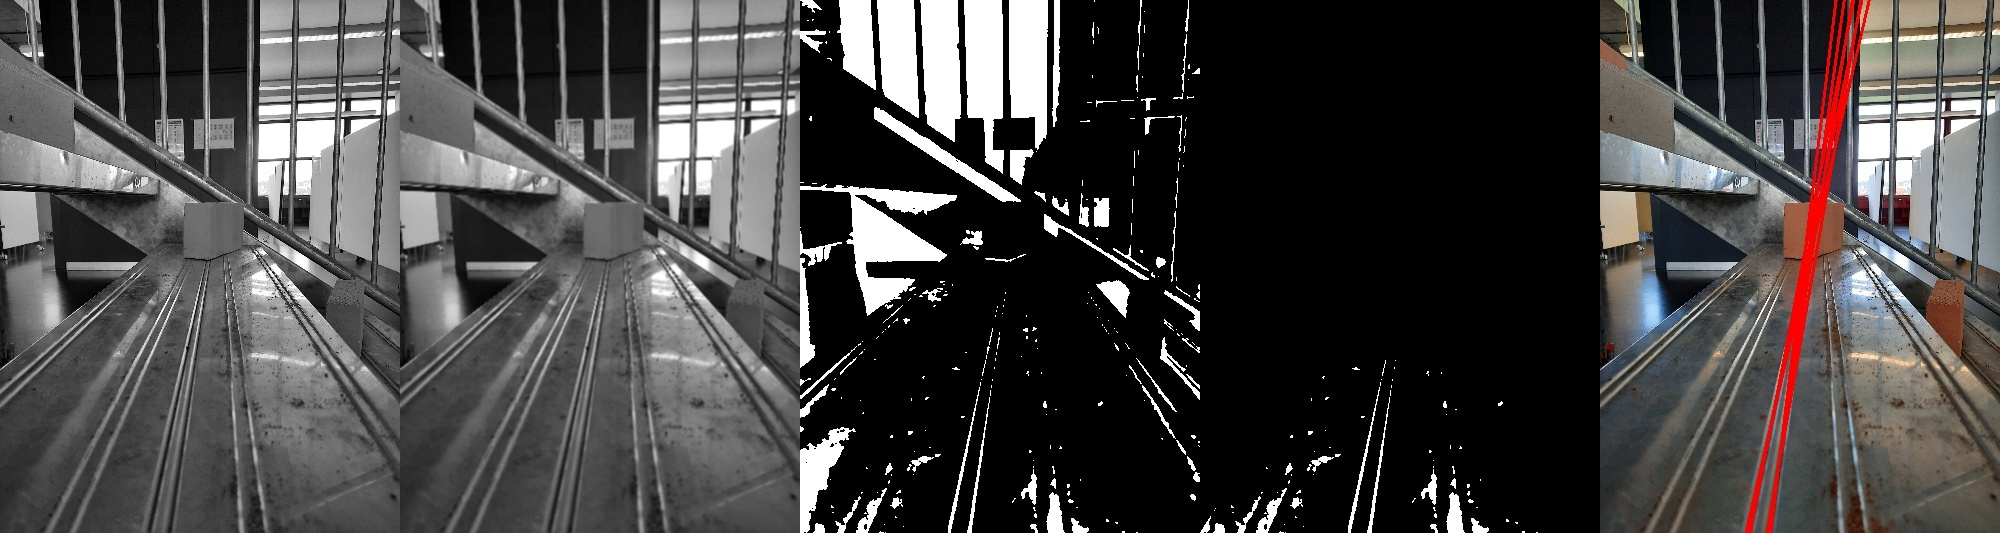
\includegraphics[width=1.0\textwidth]{img/orientierung-treppenstufe/collageThresh.jpg}
  \centering
  \caption{Bilverarbeitungschritte des Funktionsmusters für die Orientierung auf einer Treppenstufe mit thresholding}
  \label{fig:bildverarbeitungsschritte-threshold}
\end{figure}
  
\newpage
\subsubsection{Zeitmessung}
Um ein Gefühl für die Laufzeit solcher Bildverarbeitungen und für die Laufzeit dieses Funktionsmusters zu entwickeln, werden zehn Zeitmessungen erstellt (Tabelle \ref{tab:zeitmessung-bildverarbeitung}. Diese werden auf einem Microsoft Surface Book 2 durchgeführt. Die effektive Laufzeit auf dem Zielsystem (Raspberry Pi) kann also stark variieren.

\begin{center}
\begin{table}[H]
    \begin{tabular}{l|l|l|l|l|l|l|l|l|l|l}
        \textbf{Durchlauf} & 1 & 2 & 3 & 4 & 5 & 6 & 7 & 8 & 9 & 10 \\
        \textbf{Zeit [ms]} & 262.88 & 204.04 & 205.01 & 205 & 212.01 & 209.56 & 205 & 206 & 206.04 & 206 \\
        \textbf{Durchschnitt [ms]} & 212.15 \\
    \end{tabular}
    \caption{Zeitmessung des Algorithmus für die Orientierung auf einer Treppenstufe}
    \label{tab:zeitmessung-bildverarbeitung}
\end{table}
\end{center}

Eine Raspberry Pi Kamera liefert 30 Bilder pro Sekunde. Somit wäre es nicht im entferntesten möglich, die Positionsbestimmung auf jedem einzelnen Bild durchzuführen. Hierfür müsste der Algorithmus stark optimiert werden. Eine Möglichkeit zur Optimierung wäre, die Maskierung bereits zu Beginn durchzuführen, wie im Kapitel \ref{sec:aufbereitung-der-bilder} (Aufbereitung der Bilder) kurz erwähnt.
  
\subsubsection{Fazit}
Es ist möglich, auf dieser Treppe mithilfe der Kamera sinnvolle Kanten auszulesen, welchen der Roboter folgen kann. Mit beiden verschiedenen Algorithmen (Canny Edge und Thresholding) werden ähnliche Ergebnisse erzielt. Der Mittelpunkt der Treppe, an welchem sich der Roboter orientieren kann, wird erkannt. Wenn sich dieser Mittelpunkt im Bild nach Rechts bewegt, ist dies ein Anzeichen dafür, dass der Roboter nach Links abdriftet und nach rechts gegensteuern muss. Anhand des Winkels der Mittelpunktgerade kann die Ausrichtung des Roboters überprüft werden. Wenn die Gerade beispielsweise einen Winkel von 60$^\circ$
 hat, ist bekannt, dass der Roboter 30$^\circ$ nach rechts geneigt auf der Treppe steht.
Es ist noch nicht klar, welcher Algorithmus besser geeignet ist. Es wäre allenfalls auch eine Kombination der beiden denkbar, um verschiedene Lichtverhältnisse besser abfangen zu können.

\newpage
\subsection{Treppensteigen Prototyp 1}
Das Lego-Mock-Up, das erstellt wurde, um die Hubbewegungen von Hand simulieren zu können, soll dazu verwendet werden, die Hubbewegungen zu automatisieren. Es wird nur eine Seite der Treppensteigkomponenten aufgebaut. 

Der erste Prototyp, welcher in Abbildung \ref{fig:prototyp-treppensteigen} gezeigt wird, diente dazu das Funktionsprinzip zu überprüfen. Es muss überprüft werden, ob die Standfüsse und die Verbindungsleisten unabhängig mit zwei Motoren gedreht werden können. 

\subsubsection{Mechanische Komponenten}
Das Lego-Mock-Up wird für den Prototypenbau verkleinert, da der eingekaufte Modelbauzahnriemen nicht ganz den ersten Massabschätzungen entsprach. Die Zahnriemenräder, welche die Abbildung \ref{fig:3d-gedrucktes-zahnriemenrad} veranschaulicht, werden selber 3D-gedruckt. Das Antriebsrad konnte so direkt mit einem Zahnrad kombiniert werden. Auch das Antriebsrad kann direkt mit einer Legowelle gedruckt werden. Der Grundkörper, die Standfüsse und die Verbindungsleisten werden aus Legotechnik aufgebaut.\\

\begin{figure}[H]
  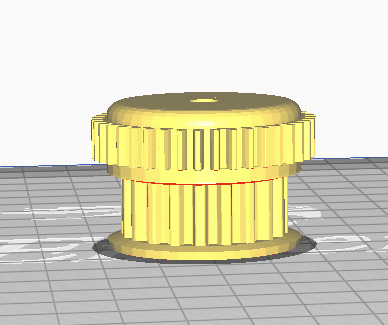
\includegraphics[width=0.6\textwidth]{img/Zahnrad gedruckt.JPG}
  \centering
  \caption{3D-gedrucktes Zahnriemenrad mit aufgesetztem Zahnrad}
  \label{fig:3d-gedrucktes-zahnriemenrad}
\end{figure}

\begin{figure}[H]
  \includegraphics[width=0.6\textwidth]{img/Prototyp Übersicht.png}
  \centering
  \caption{Protototyp Treppensteigen}
  \label{fig:prototyp-treppensteigen}
\end{figure}

\subsubsection{Elektrische Komponenten}
Um die Bewegung der Arme ausführen zu können, werden zwei Getriebemotoren verwendet. Diese Motoren werden durch eine H-Brücke angesteuert. Die Ansteuerung der H-Brücken übernimmt ein Raspberry Pi 4.

\begin{figure}[H]
  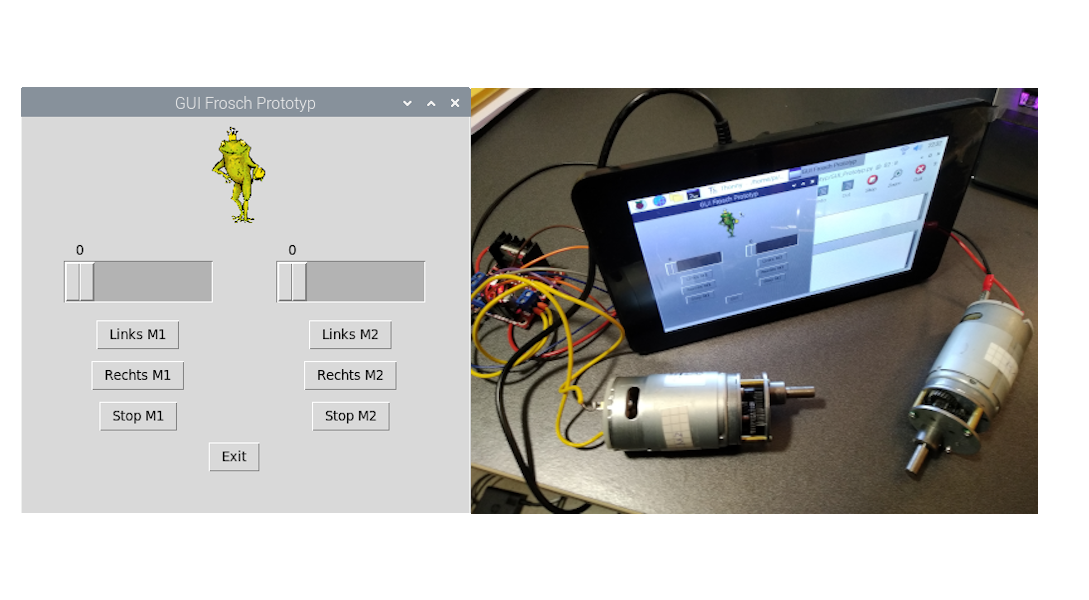
\includegraphics[width=\textwidth]{img/Funktionsmuster Treppensteigen/GUI.png}
  \centering
  \caption{GUI und Elektrische Komponenten des Prototyps}
  \label{fig:gui-prototyp}
\end{figure}

\newpage

Um die Geschwindigkeit der Motoren individuell anpassen zu können, generiert der Raspberry Pi ein PWM-Signal für die H-Brücke. Dieses PWM-Signal kann in einem GUI (siehe Abbildung \ref{fig:gui-prototyp}) mittels Slider von 0 bis 100\% verstellt werden. 
Des Weiteren hat man die Möglichkeit auf dem GUI die Drehrichtung der einzelnen Motoren nach links und nach rechts zu wählen, sowie einzeln zu stoppen.

\subsubsection{Test}
Es wird geprüft, ob sich der Standfuss mit dem Zahnriemen drehen lässt und ob mit dem zweiten Motor die Verbindungsleiste gedreht werden kann. Diese Versuche werden zuerst einzeln gemacht, um die jeweilige Funktion zu testen. Zum Schluss wird noch versucht, mit der Verbindungsleiste eine Umdrehung zu machen und dabei den Standfuss horizontal zu halten. Die Abbildung \ref{fig:test-prototyp-treppensteigen} zeigt den Prototypen während den Tests.

\begin{figure}[H]
  \includegraphics[width=0.8\textwidth]{img/Testversuch.png}
  \centering
  \caption{Test des Funktionsprinzips}
  \label{fig:test-prototyp-treppensteigen}
\end{figure}

\subsubsection{Fazit}
Mit diesem Prototypen sollten die Hubbewegungen automatisiert werden. Dies ist so nicht gelungen, jedoch konnte mit dem Prototyp das Funktionsprinzip überprüft werden.

Nach den ersten Tests wird klar, dass das Funktionsprinzip funktioniert. Es gilt jedoch einige Faktoren zu beachten. Die grösste Erkenntnis beim Bau des Prototypen ist, dass zwei Motoren notwendig sind. Je ein Motor wird für eine Drehung einer Achse benötigt. Diese Motoren treiben beide Seiten synchron an. Die Kraftübertragung wurde mithilfe des Prototyps getestet.

Der Bau des Prototypen für das Treppensteigen war wichtig und hat geholfen das Funktionsprinzip aufzubauen und zu verstehen.

\newpage

\subsection{Treppensteigen Prototyp 2}
Da mit dem ersten Prototypen nur das Funktionsprinzip überprüft werden konnte, brauchte es einen zweiten Prototypen, um die erste Hubbewegung zu simulieren, da sie die wichtigste Hubbewegung beim besteigen der Treppe ist. Es gilt zu überprüfen, ob die erste Hubbewegung überhaupt machbar ist. Der zweite Prototyp ist in Abbildung \ref{fig:prototyp-2-treppensteigen} ersichtlich.

\begin{figure}[H]
  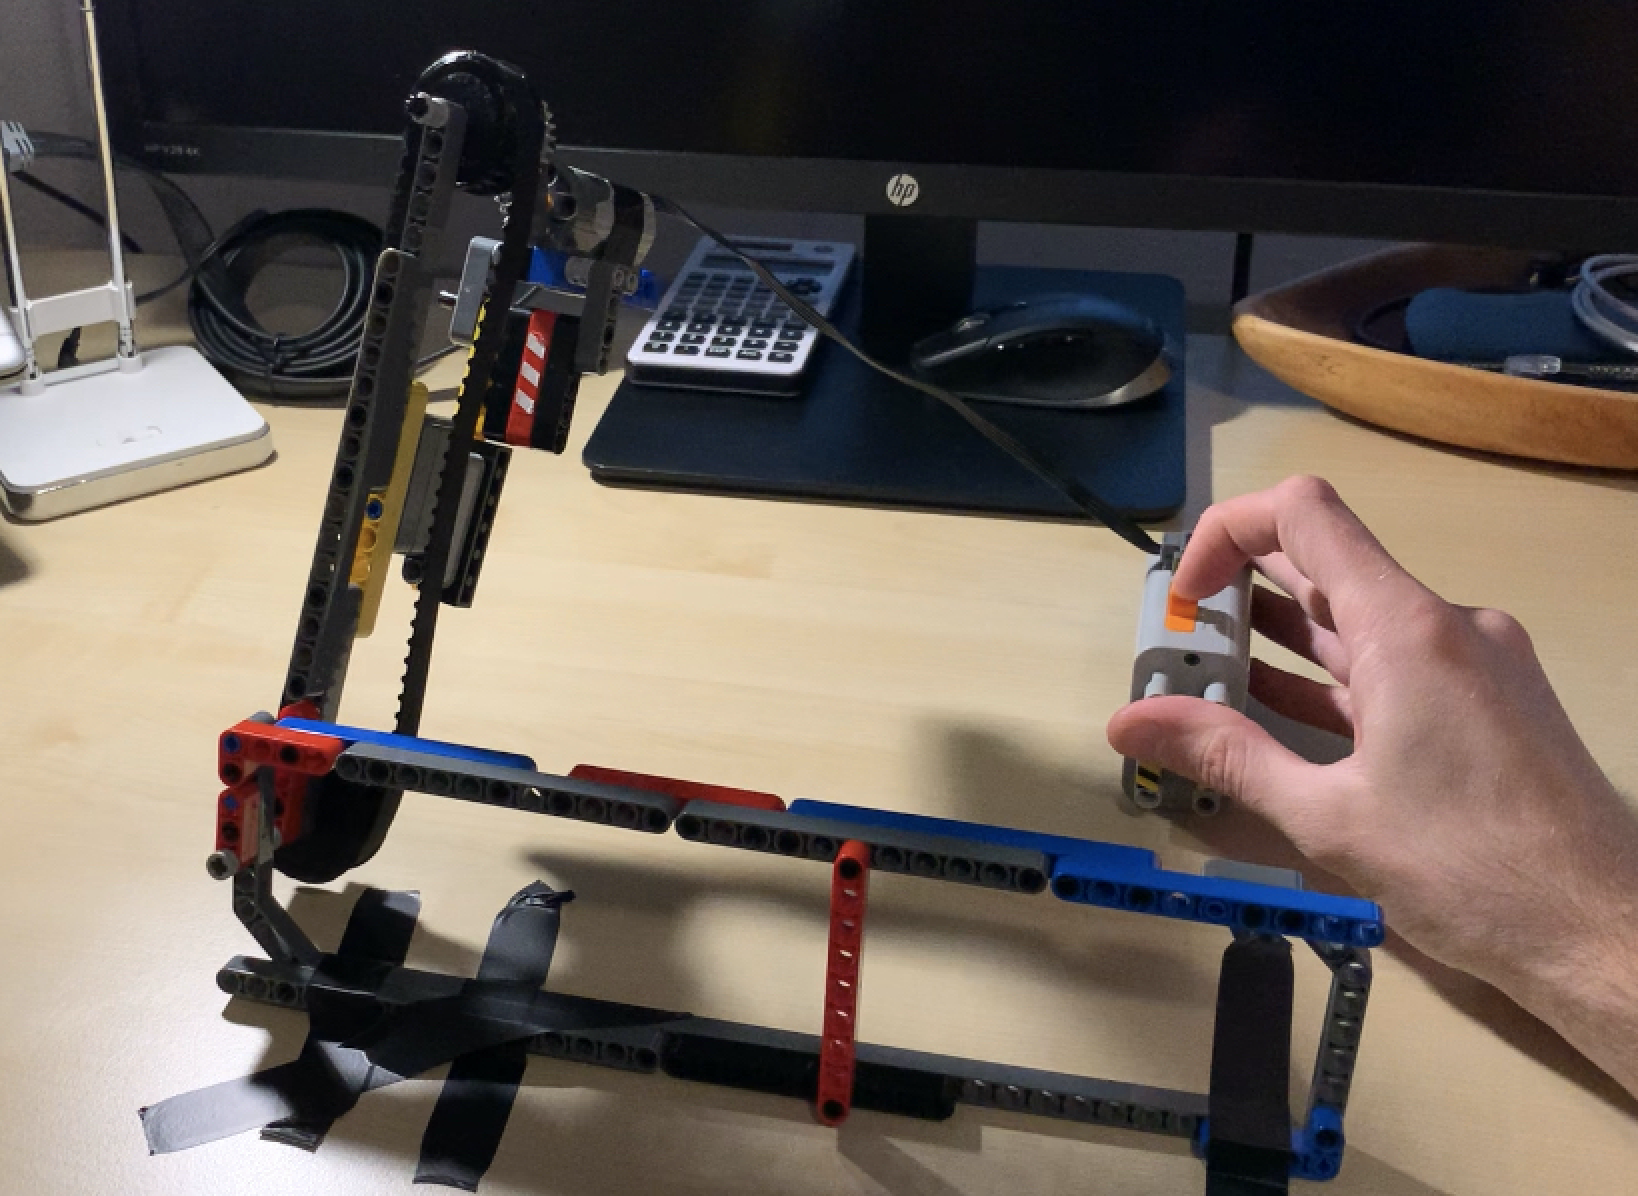
\includegraphics[width=0.8\textwidth]{img/Test 1. Hub.png}
  \centering
  \caption{Test 1. Hubbewegung}
  \label{fig:prototyp-2-treppensteigen}
\end{figure}

\subsubsection{Fazit}
Es konnte gezeigt werden, dass die erste Hubbewegung umsetzbar ist. Die Bewegung funktioniert mit dem Zahnriemen als Kraftübertragung.

\newpage
\subsection{Fortbewegung Prototyp}
Für die Fortbewegung und Navigation des Roboters werden zwei voneinander unabhängige drehbare Räder verwendet. Damit der Grundkörper gerade liegt und nicht den Boden berührt, werden gegenüber der Räder zwei Halbkugelstützen verbaut.
Dieses System wurde gewählt, da es extrem simpel ist und der Roboter sich auf einem Punkt drehen kann.

Um die Funktionsweise für die Fortbewegung zu demonstrieren und erste Tests für Drehungen auf
der Treppe durchzuführen, wird ein Prototyp mithilfe von Lego Mindstorms \footnote{https://en.wikipedia.org/wiki/Lego\_Mindstorms} (siehe Abbildung \ref{fig:lego-mindstorms}) gebaut.

\begin{figure}[H]
  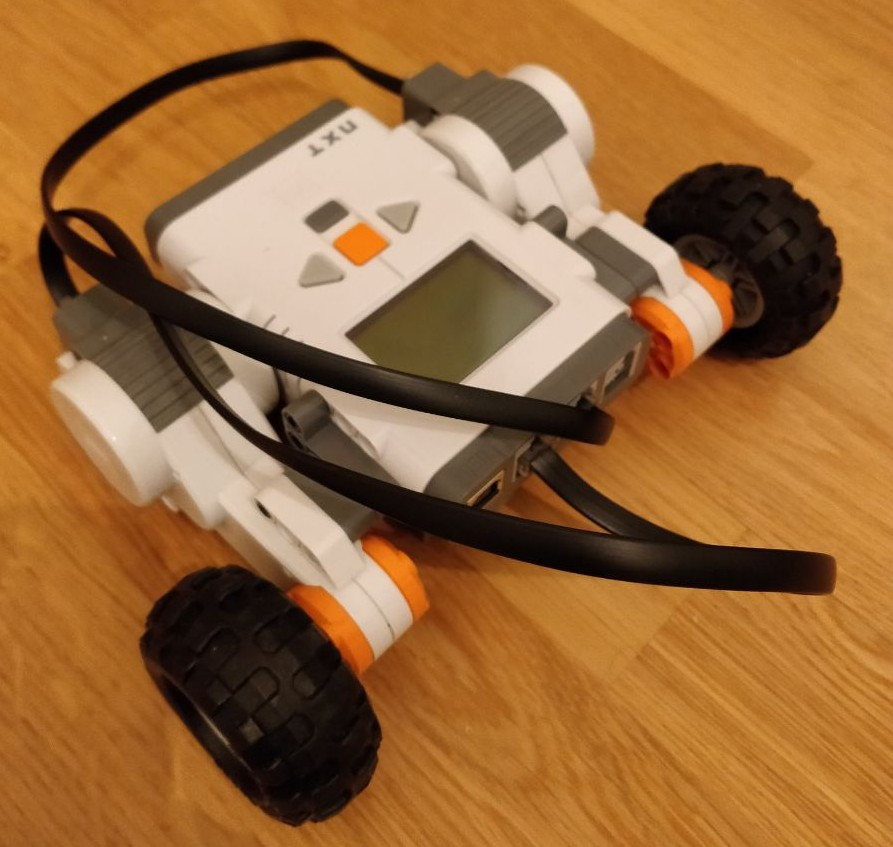
\includegraphics[width=0.8\textwidth]{img/Fortbewegung/fortbewegung.png}
  \centering
  \caption{Fortbewegungsprinzip mit Lego Mindstorms}
  \label{fig:lego-mindstorms}
\end{figure}




